\section{Introducción}

El plan arranca de una decisión del grupo: \textbf{medir} si un contrato OpenAPI bancario y un
\ServiceDomain{} BIAN emparejado hablan del mismo negocio, y hacerlo con un número reproducible,
no con una revisión ad hoc.

OpenAPI es el archivo YAML o JSON con \textit{paths}, verbos HTTP y \textit{schemas} (Casas et al.,
2021; Santos et al., 2020). BIAN ---\textit{Banking Industry Architecture Network}--- parte el
negocio en \ServiceDomain{}s (pagos, cuentas) con \textit{behaviors} y \textit{business objects}
(Farzi, 2021). Un equipo publica el contrato; otro conserva el modelo de referencia. Casi nunca hay
una métrica que los cruce \textbf{antes} del despliegue.

Llamamos \textbf{alineación} a ese cruce. El producto es un modelo de puntuación:
\SemanticScore{} (S), \StructuralScore{} (E), \CoverageScore{} (C) y
\AlignmentScore{} $= \alpha S + \beta E + \gamma C$ con $\alpha + \beta + \gamma = 1$
(§1.4 y Fig.~\ref{fig:alignment-score}).

El sector ya mostró el costo de no hacerlo. TSB (2018) y el \textit{open banking} británico
(CMA, 2016) aparecen en §\ref{sec:problematica} como síntomas; el objeto ---el contrato, no el
banco--- se fija en §\ref{sec:objeto-estudio}; el problema tecnológico, en
§\ref{sec:planteamiento}.

Guía~1 \textbf{diseña} el procedimiento y lo deja trazado en el Anexo~C. Construir el parser y
correr scores queda para Tesis~2 (§\ref{sec:alcances}).

La \Cref{fig:contexto} sitúa el flujo: APIs bancarias, BIAN como referencia, OpenAPI como entrada,
S/E/C como salida.

\begin{figure}[H]
  \centering
  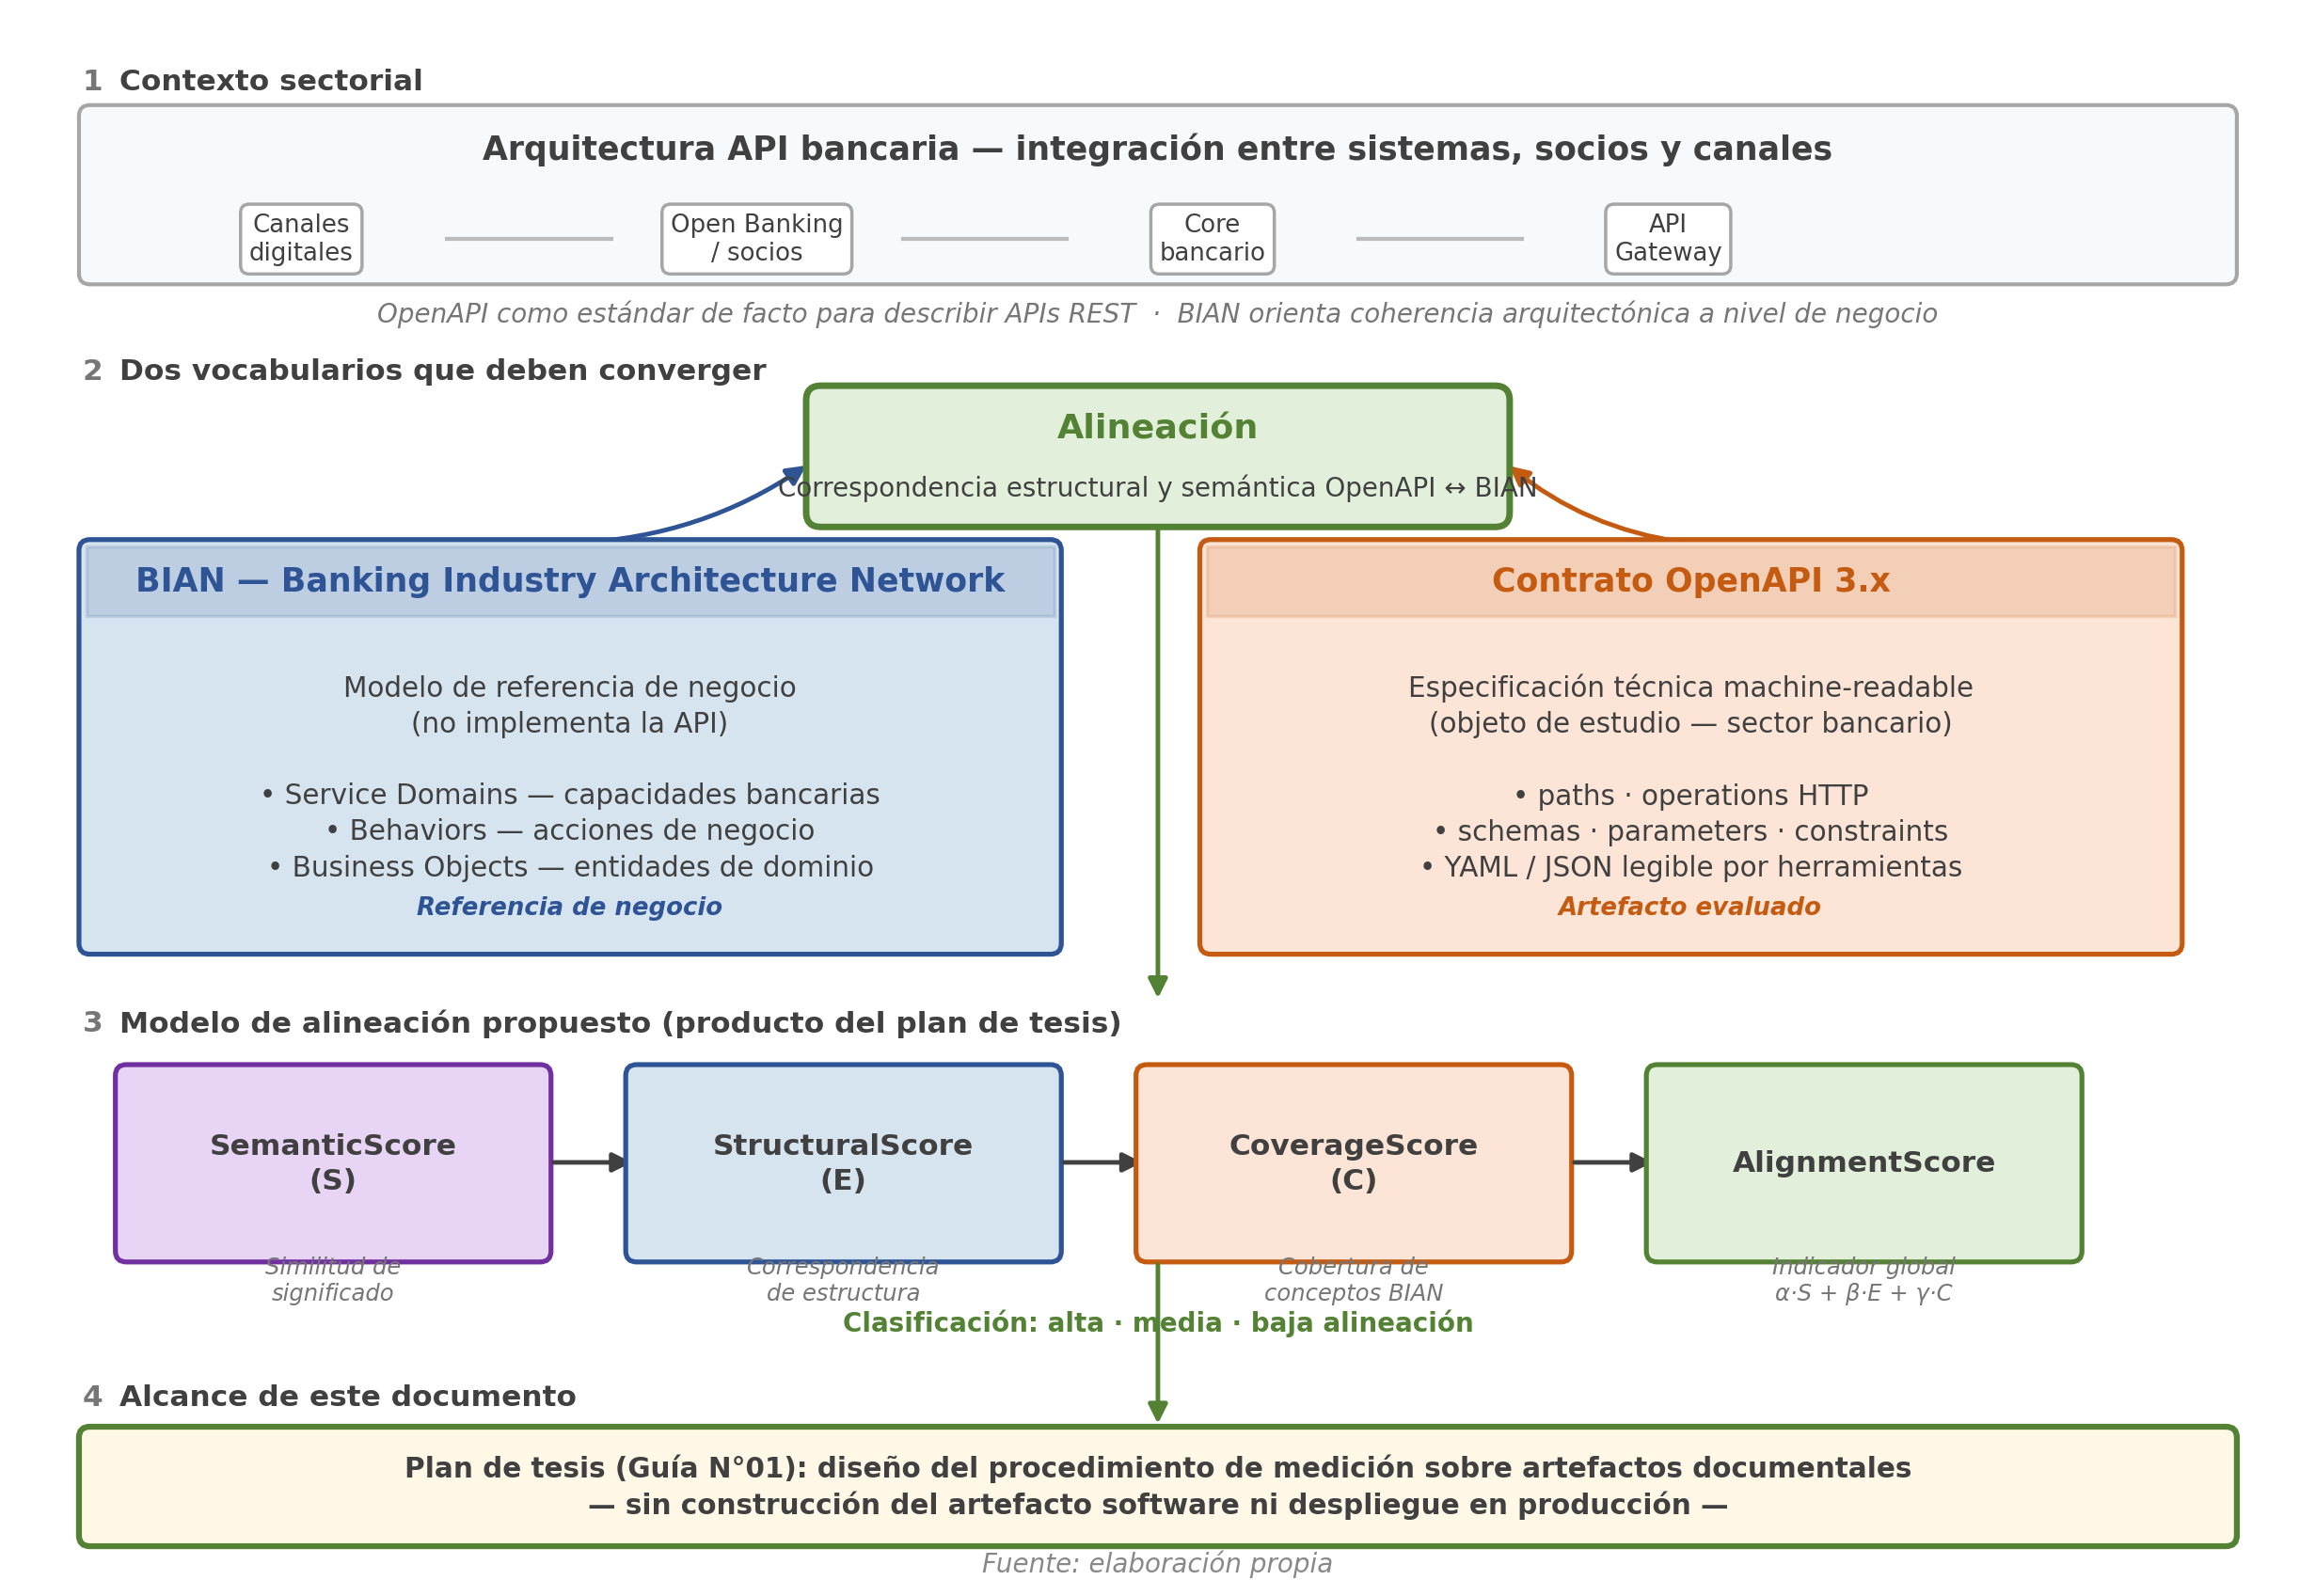
\includegraphics[width=0.92\textwidth]{Figura_01_Contexto}
  \caption{Contexto: arquitectura API bancaria, BIAN, OpenAPI y modelo S/E/C}
  \label{fig:contexto}
\end{figure}

Sigue la situación real (§\ref{sec:problematica}), luego el planteamiento y el objeto. Objetivos,
marco y método ocupan los capítulos~\ref{cap:objetivos}--\ref{cap:metodologia}; el Capítulo~5
administra el plan.
